% Copyright (C) 2005-2015 Airbus - EDF - IMACS - Phimeca
% Permission is granted to copy, distribute and/or modify this document
% under the terms of the GNU Free Documentation License, Version 1.2
% or any later version published by the Free Software Foundation;
% with no Invariant Sections, no Front-Cover Texts, and no Back-Cover
% Texts.  A copy of the license is included in the section entitled "GNU
% Free Documentation License".
\renewcommand{\filename}{docUC_StocProc_Process.tex}
\renewcommand{\filetitle}{UC : Manipulation of a process}

% \HeaderNNIILevel
\HeaderIILevel
%\HeaderIIILevel

\label{UCprocess}


\index{Stochastic Process!Process Manipulation}



The objective here is to manipulate a multivariate stochastic process $X: \Omega \times \cD \rightarrow \Rset^d$, where $\cD \in \Rset^n$ is discretized on the mesh $\cM$.

A continuous realization from the process $X$ is defined as the numerical math function defined for a given $\omega \in \Omega$:
\begin{align}
  X(\omega):  \cD \rightarrow \Rset^d
\end{align}
According to the process, the continuous realizations are build :
\begin{itemize}
\item either using a dedicated functional model if it exists: e.g. a functional basis process (see Figures \ref{continuousReal1} to \ref{FBP});
\item or using an interpolation from a discrete realization of the process on $\cM$: in  dimension $d=1$,  a linear interpolation and in dimension $d \geq 2$,  a piecewise constant function (the value at a given position is equal to the value at the nearest vertex of the mesh of the process).
\end{itemize}
We get a continuous realization  thanks to the method \emph{getContinuousRealization}. \\



In addition, it is possible:
\begin {itemize}
\item to extract its marginal process  for $ j \in [0,d-1]$ : $X_j: \Omega \times \cD \rightarrow \Rset$ thanks to the method \emph{getMarginalProcess};
\item to get one or several realization(s) of the process, thanks to the methods \emph{getRealization}, \emph{getSample};
\item to get its mesh, thanks to the method \emph{getMesh} and its time grid, thanks to the method \emph{getTimeGrid} when the mesh can be interpreted as a regular time grid;
\item to check wether the process is normal or stationary, thanks to the methods \emph{isNormal} and \emph{isStationary}.
\end{itemize}

\requirements{
  \begin{description}
  \item[$\bullet$] a stochastic process {\itshape myProcess}
  \item[type:]  Process
  \end{description}
}
             {
               \begin{description}
               \item[$\bullet$] a time grid or a mesh: {\itshape myTimeGrid, myMesh}
               \item[type:]  RegularGrid, Mesh
               \end{description}

               \begin{description}
               \item[$\bullet$] a field or a  sample of fields :: {\itshape myField, myFieldSample}
               \item[type:]  Field, ProcessSample
               \end{description}

               \begin{description}
               \item[$\bullet$] a stochastic process {\itshape myMarginalProcess}
               \item[type:]  Process
               \end{description}

               \begin{description}
               \item[$\bullet$] a continuous realization: {\itshape myContReal}
               \item[type:] NumericalMathFunction
               \end{description}
             }

             \textspace\\
             Python script for this Use Case :
             \inputscript{script_docUC_StocProc_Process}

             Figures \ref{continuousReal1} and \ref{continuousReal2} draw two continuous realizations of the functional basis process  $X: \Omega \times [-4,4]^2 \rightarrow \Rset$ defined by:
             \begin{align}
               X(\omega,(x,y))=\sum_{i=1}^3 \sum_{j=1}^3 \alpha_{i,j}(\omega)\sin(ix) \sin(jy)
             \end{align}
             where the random variables $\alpha_{i,j}$ are iid according to the standard normal distribution.


             \begin{figure}[H]
               \begin{minipage}{9cm}
                 \begin{center}
                   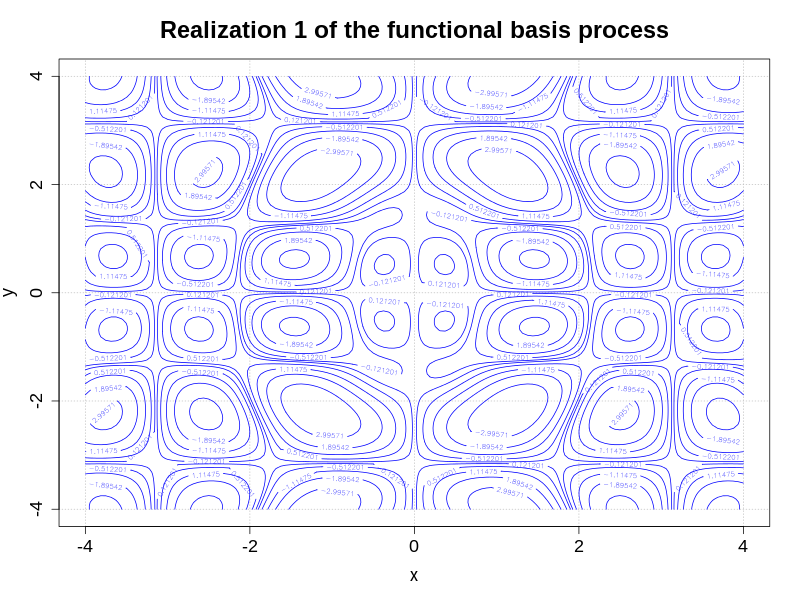
\includegraphics[width=7cm]{Figures/continuousReal1.png}
                   \caption{One realization of the functional basis process.}
                   \label{continuousReal1}
                 \end{center}
               \end{minipage}
               \hfill
               \begin{minipage}{9cm}
                 \begin{center}
                   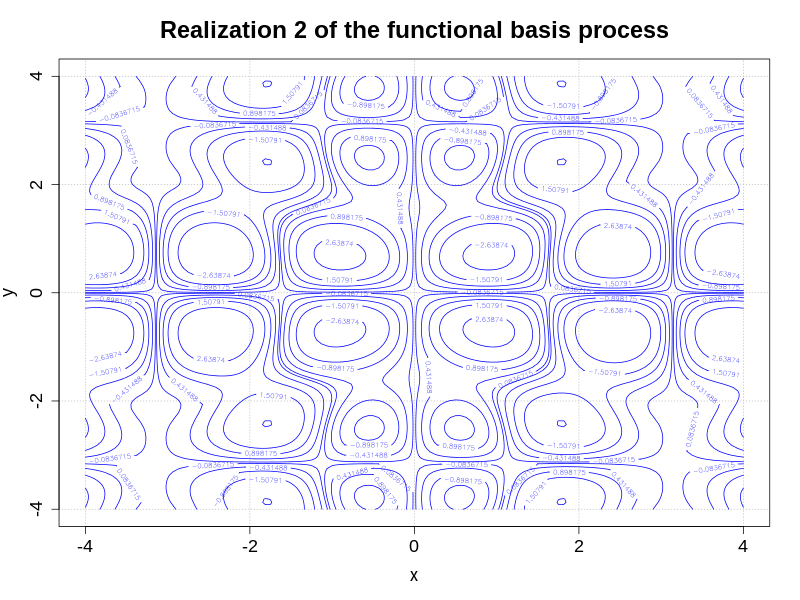
\includegraphics[width=7cm]{Figures/continuousReal2.png}
                   \caption{One realization of the functional basis process.}
                   \label{continuousReal2}
                 \end{center}
               \end{minipage}
             \end{figure}

             In Figure \ref{FBP}, we draw one realization versus one continuous realization of the functional basis process $X: \Omega \times [0,1] \rightarrow \Rset$ defined by:
             \begin{align}
               X(\omega, x)=\sum_{i=1}^{10} \Xi_{i}(\omega)\sin(2i\pi x)
             \end{align}
             on the regular grid  of $[0,1]$ discretized with 21 points, where the coefficient s $\Xi_i$ are independent and respectively distributed according to $Normal(0,\sigma=1.0/i)$.\\
             When we ask for a realization, we get a field (each vertex $x_k$ of the mesh is associated to a value of the process $X$). The method \textit{draw} draws a linear interpolation of the values: see the blue line.\\
             When we ask for a continuous realization, we get a function $X(\omega): [0,1] \rightarrow \Rset$ defined by:
             \begin{align}
               X(\omega)(x)=\sum_{i=1}^{10} \xi_{i}(\omega)\sin(2i\pi x)
             \end{align}
             where $ \xi_{i}= \Xi_{i}(\omega)$.  The method \textit{draw} draws the graph of the function, which is continuous and can be evaluated on other points than those of the mesh: see the red line.


             \begin{figure}[H]
               \begin{center}
                 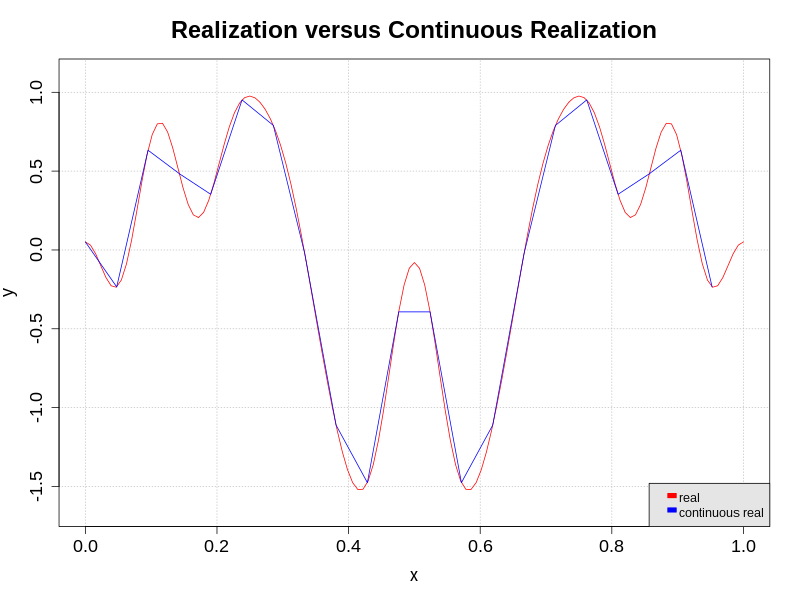
\includegraphics[width=7cm]{Figures/FuncBasProc_real.png}
                 \caption{One realization versus one continuous realization of the function basis process $X$.}
                 \label{FBP}
               \end{center}
             \end{figure}


             In Figure \ref{TGP}, we define a normal process of dimension 1 which covariance model is $Exponential(a,\lambda)$ with $a=1.0$ and $\lambda=4.0$. The associated mesh is the regular grid of $[0,1]$ discretized with 21 points.\\
             When we ask for a realization, we get a field and the method \textit{draw} draws a linear interpolation of the values: see the blue line.\\
             When we ask for a continuous realization, we get a function $X(\omega): [0,1] \rightarrow \Rset$ which is built using a linear interpolation of the values of the field: see the red line. \\
             In that case, both methods \emph{getRealization} and \emph{getContinuousRealization} lead to the same graph.


             \begin{figure}[H]
               \begin{center}
                 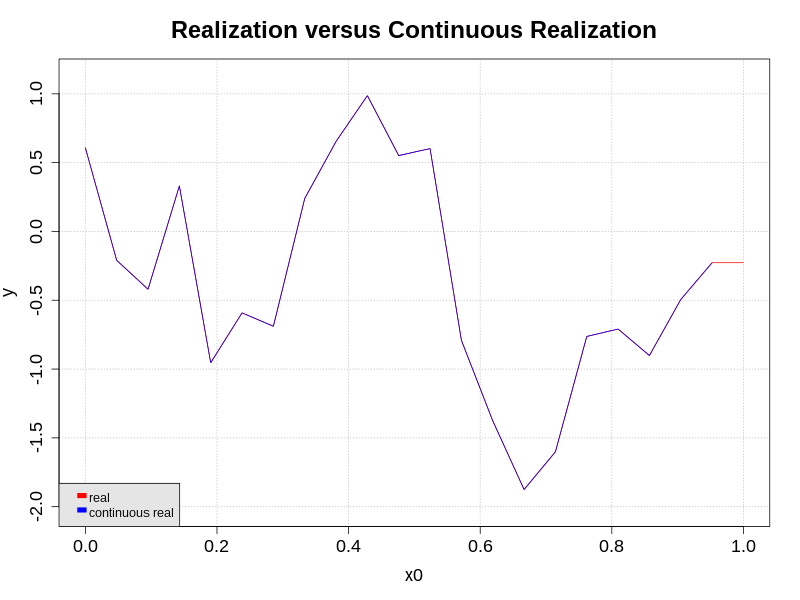
\includegraphics[width=7cm]{Figures/TNProc_real.png}
                 \caption{One realization versus one continuous realization of temporal normal process of dimension 1.}
                 \label{TGP}
               \end{center}
             \end{figure}
